\section{Introdução}
Trataremos aqui sobre uma rede neural do tipo "Adaline".

Suas principais características são: tem a função de ativação do tipo linear e a quantidade de ciclos é determinada pela precisão, um parâmetro que envolve a variação dos erros quadráticos da saída de cada ciclo.

Para este trabalho utilizaremos uma aplicação prática dos Adalines, um sistema recebe três entradas ($x_{1} \cdots x_4)$ as quais servem de parâmetro para ativar duas válvulas, então estes dados passarão por um tratamento através do Adaline e retornar valores bipolares, 1 (ativa a válvula A) ou -1 (ativa a válvula B).

\begin{figure}[H]
	\centering
	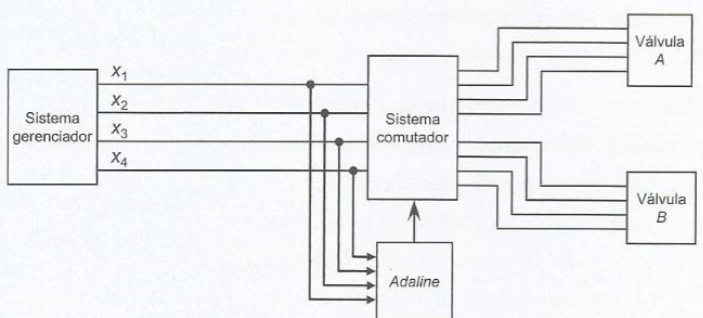
\includegraphics[scale = 0.6]{imagens/visual}
	\caption{Esquema visual do sistema.}
\end{figure}